\documentclass{ctexart}

\usepackage{amssymb}
\usepackage{amsmath}
\usepackage{enumerate}
\usepackage[numbers]{natbib} 
\usepackage{geometry}
\geometry{left=3.0cm,right=3.0cm,top=2.5cm,bottom=2.5cm}
\usepackage{fancyhdr}
\pagestyle{fancy}
\lhead{}
\rhead{}
\setlength{\headheight}{15mm}
\fancyhead[C]{
	\begingroup
	\setlength{\tabcolsep}{10pt} % Default value: 6pt
	\renewcommand{\arraystretch}{1.5} % Default value: 1
	\begin{tabular}{ccc}
		& \large{\textbf{傅立叶光学实验报告}} &  \\
		少年班学院 \qquad \qquad & 刘子安 PB20000069 & \qquad \today
	\end{tabular}
	\endgroup
}   %在此处插入作者信息,改变页眉,此页眉是由我设计的,类似于实验报告纸
\fancyfoot[C]{ 第 {\thepage} 页,共 \pageref{unknown} 页}
\renewcommand{\headrulewidth}{0pt}

\usepackage{graphicx}

\usepackage{siunitx}

\begin{document}
	
\subsection*{实验目的}
\begin{itemize}
    \item 知道什么是空间频谱,以及如何使用透镜观察物面的空间频谱。
    \item 了解空间滤波的概念,知道在空间频谱面上进行空间滤波操作与像面的关系。
    \item 使用透镜观察物面的空间频谱与夫琅禾费衍射的关系。
\end{itemize}
\subsection*{实验原理}
我们知道一个复变函数$f(x,y)$的傅立叶变换为:
$$
F(u, v) = \mathfrak{F} \{f(x, y)\} = \iint f(x, y) \exp[-i2\pi(ux+vy)]dxdy
$$

$F(u,v)$叫作$f(x,y)$的傅立叶变换函数或者频谱函数,$f(x, y)$叫做原函数,也可以通过求$F(u, v)$的逆傅立叶变换得到原函数$f(x, y)$:
$$
f(x, y) = \mathfrak{F}^{-1}\{F(u, v)\} = \iint F(u, v)\exp{[i2\pi(ux+vy)]}dudv
$$

在光学成像的过程中如果将一个平面图形放在一个理想的透镜(傅立叶变
换透镜)的前焦平面上,在透镜的后焦平面就可以得到它的准确的傅立叶变换,
即得到它的频谱函数。反之如果将一个平面图形的频谱放在一个理想的透镜的前
焦平面上,在透镜的后焦平面就可以得到此平面图形(不过图形的坐标要反转)。
在透镜的后焦平面上放置各种形状和大小的光阑改变图形的频谱,再对此图形用第二
个透镜成像就可以对图形进行处理,得到经过处理的图形。这个过程叫作光学信
息处理,在透镜的后焦平面上放置的光阑叫做空间滤波器。

最典型的空间滤波器包括两个透镜(光学信息处理系统或傅立叶光学变换系统)叫作4f系统,如图一所示:
\begin{figure}[htbp]
	\centering
	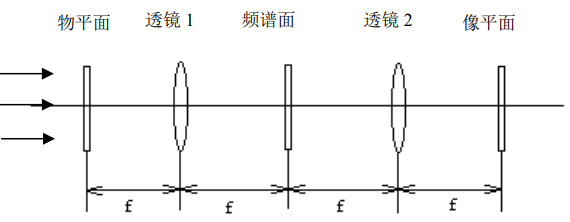
\includegraphics[scale=0.3]{1.png}
	\caption{4f 系统光路}
\end{figure}

为了实验便利,我们使用一个透镜完成空间滤波实验(阿贝成像装置):
\begin{figure}[htbp]
	\centering
	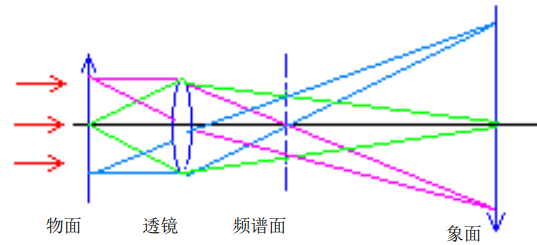
\includegraphics[scale=0.3]{2.png}
	\caption{一个透镜的傅立叶变换系统}
\end{figure}

在这种情况下,由于物面与透镜的前焦平面不重合,根据傅立叶光学的理论
可以知道在透镜的后焦平面上得到的不是物函数的严格的傅立叶变换(频谱),
不过只有一个位相因子的差别,对于一般情况的滤波处理可以不考虑。


\subsection*{实验仪器}
671nm固体激光器、扩束器、一维光栅、二维光栅、汉字屏、小透镜、傅立叶透镜、针、光屏夹。
\subsection*{实验数据分析}

\subsubsection*{测量小透镜的焦距f:}
使用如图所示的光路图:
\begin{figure}[htbp]
	\centering
	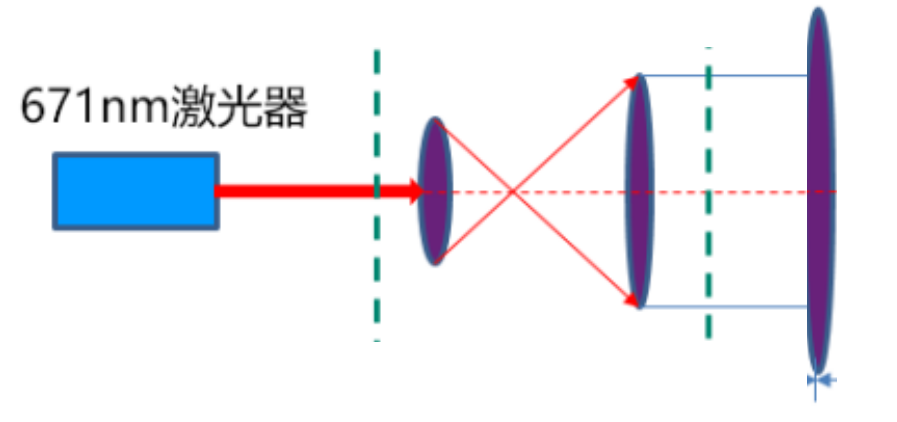
\includegraphics[scale=0.2]{3.png}
	\caption{测量小透镜的焦距f}
\end{figure}
测得小透镜的焦距为:$f = \qty{15.0}{cm}$

\subsubsection*{夫琅禾费衍射}
1.利用夫琅禾费衍射测量一维光栅常数:

按要求组装光路图,将屏幕置于频谱面,可以看到$\pm6$级左右的光斑,其中$\pm3$和
$\pm6$级光斑缺级,强度除缺级的外从0级向外依次递减。可测得小透镜到屏的距离为$l = \qty{130.0}{cm}$,
$\pm1$、$\pm2$级光斑相对0级光斑的距离为:
$$
\begin{aligned}
\Delta_{+1} &= \qty{1.05}{cm} \qquad \Delta_{+2} = \qty{2.10}{cm} \\
\Delta_{-1} &= \qty{-1.05}{cm} \quad \Delta_{-2} = \qty{-2.10}{cm}
\end{aligned}
$$

由于$\theta$很小,所以有$\sin{\theta}\backsim \tan{\theta}$,代入光栅方程$d\sin{\theta} = k\lambda$可得光栅常数$d$:
\begin{equation}
	d = \frac{k\lambda}{\tan{\theta}} = \frac{kl\lambda}{\Delta_k}
\end{equation}

将$\pm1$、$\pm2$级光斑带入方程(1)可求得:
\begin{equation}
	\begin{aligned}
		d_{-1} &= d_{+1} = \frac{kl\lambda}{\Delta_{\pm1}} = \frac{\pm1\times1.300\times6.71\times10^{-7}}{\pm1.05\times10^{-2}} = \qty{8.31e-5}{m} \\
		d_{-2} &= d_{+2} = \frac{kl\lambda}{\Delta_{\pm2}} = \frac{\pm2\times1.300\times6.71\times10^{-7}}{\pm2.10\times10^{-2}} = \qty{8.31e-5}{m}
	\end{aligned}
\end{equation}

2.二维光栅衍射

二位光栅的衍射为二维点阵,现象如图4所示。

\begin{figure}
	\centering
	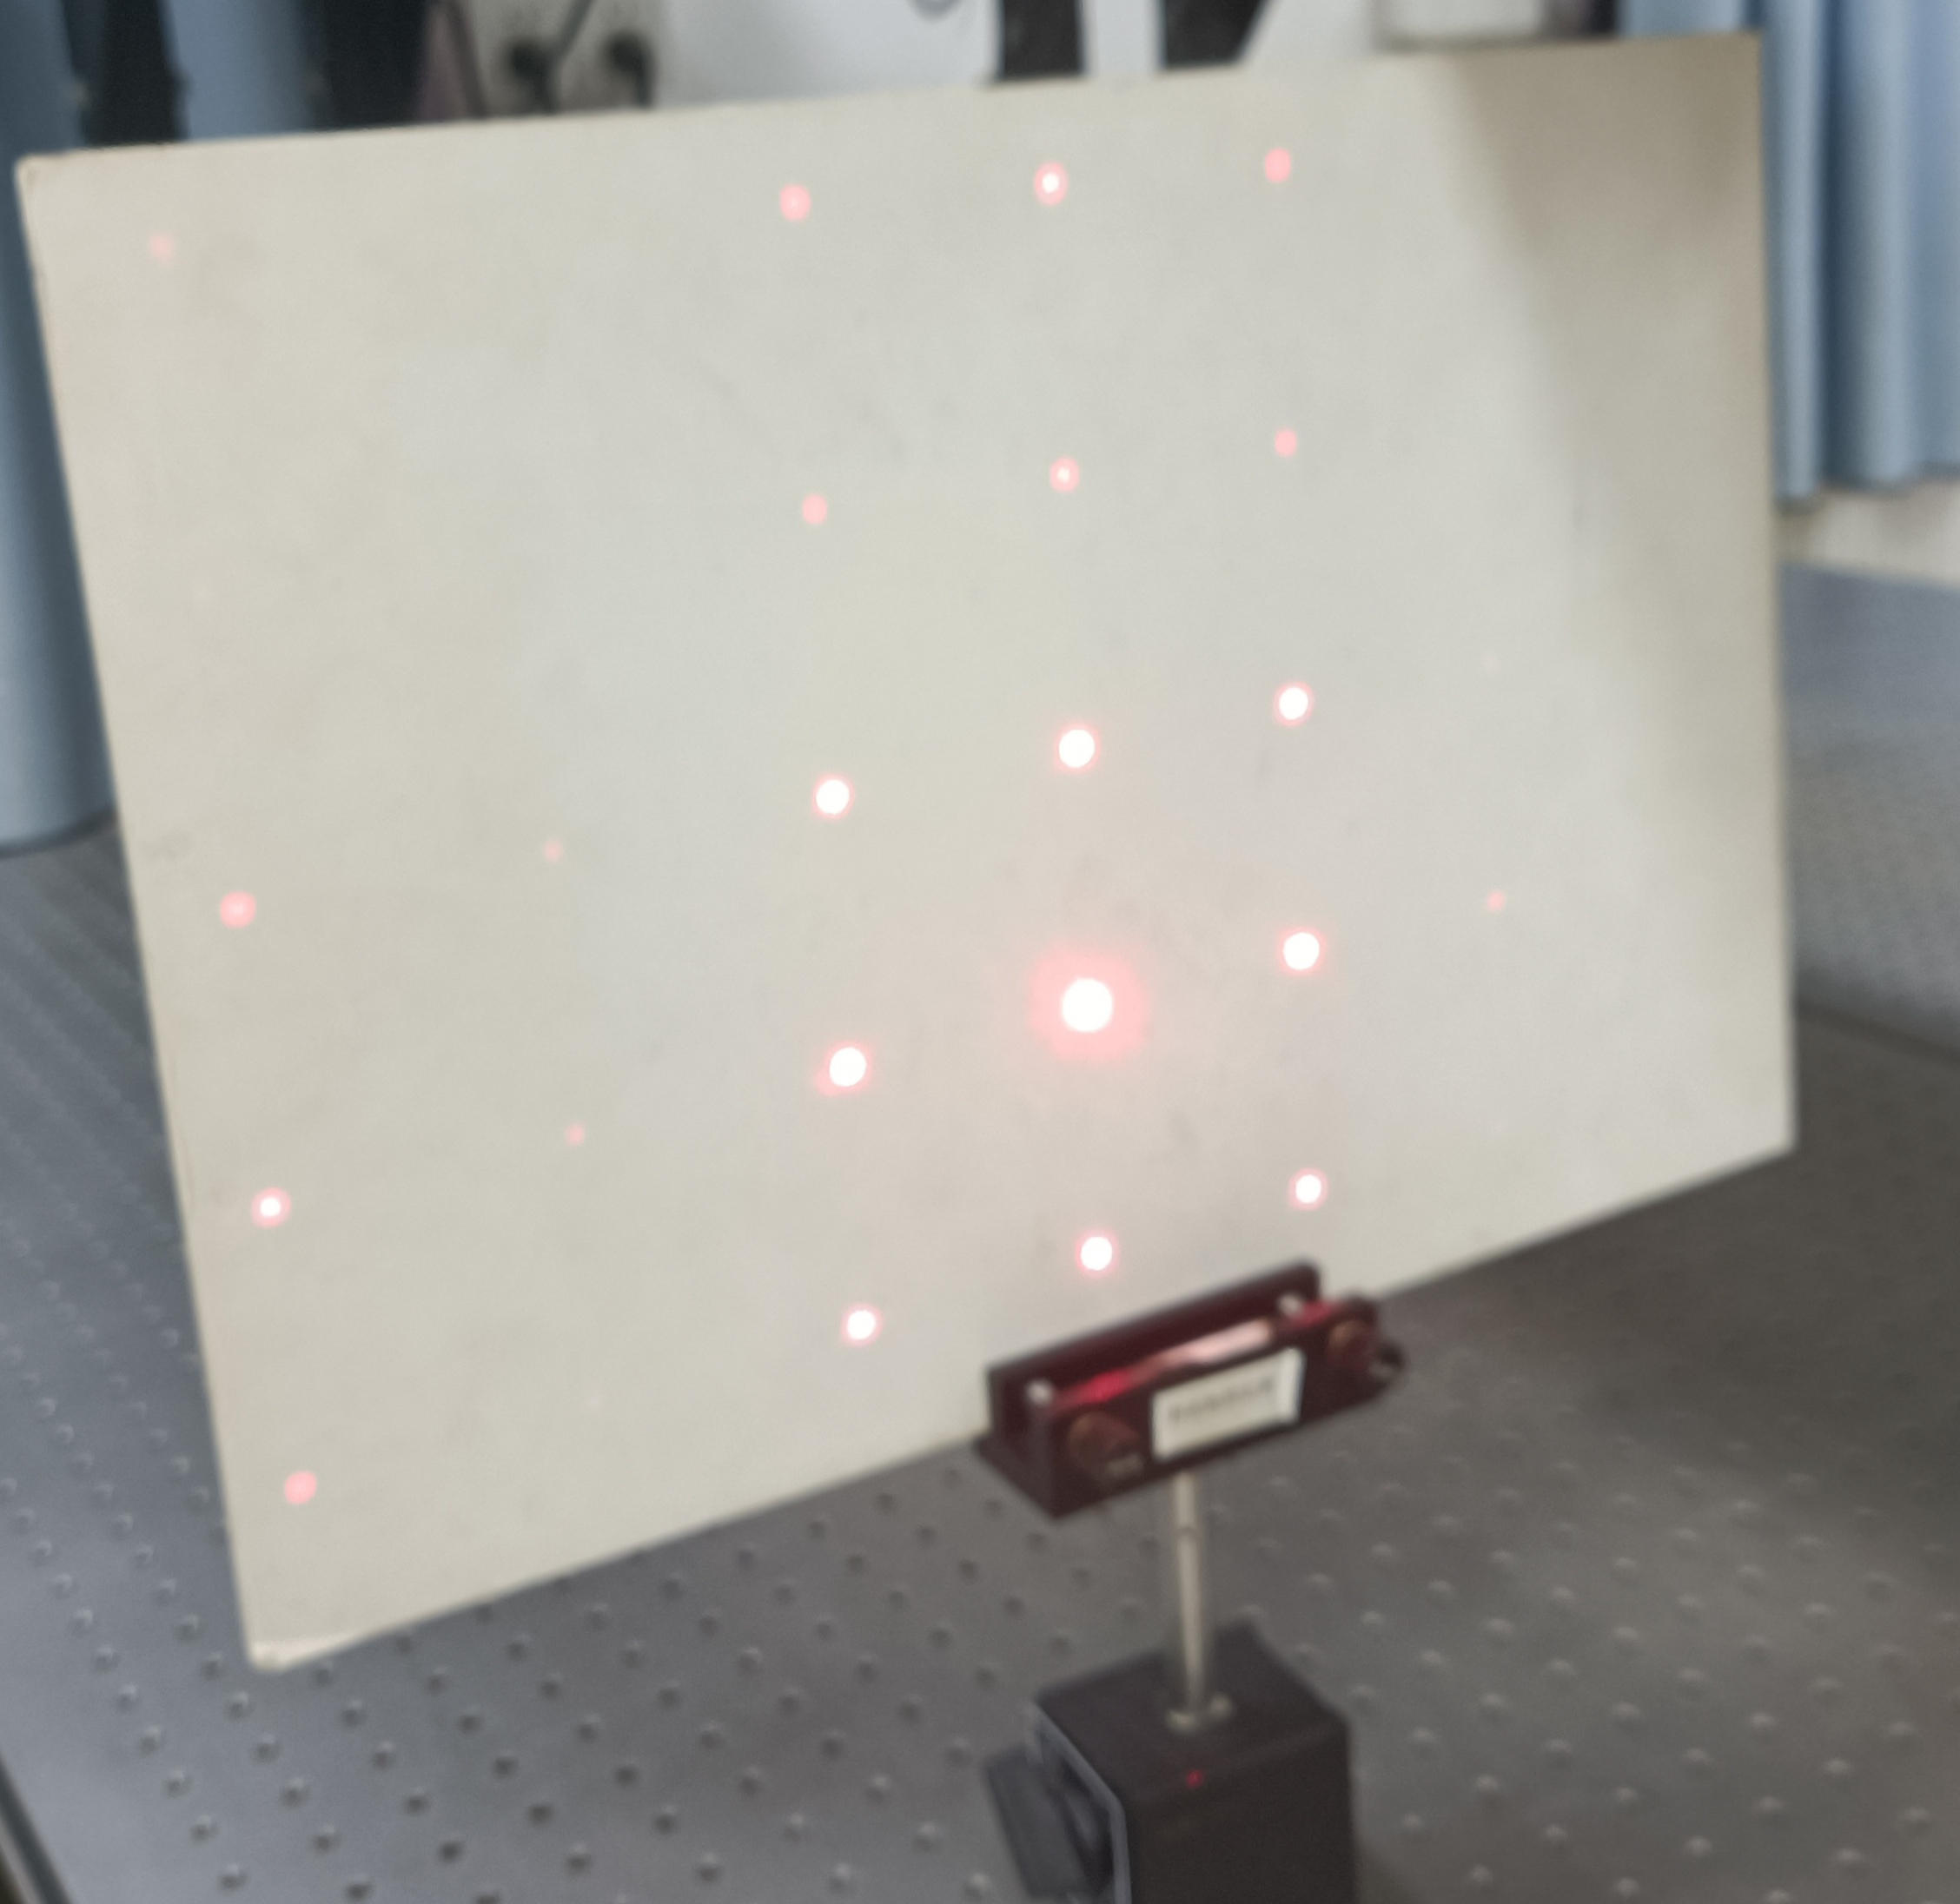
\includegraphics[scale=0.06]{4.jpg}
	\caption{二维光栅的衍射}
\end{figure}

我们可以发现,中心点的光强最大,远离中心点光强近似越来越小,每一行与每一列
都近似于一维的光栅衍射,且大概每行列级数为3的光斑强度相对较低。
\\
3.不同滤波条件下的图样
\\
(1) 一维光栅
\begin{itemize}
	\item[a.] 滤波范本只让0级通过 \par
	无法看见光栅中的条纹,仅有一个大概的轮廓。
	\item[b.] 滤波范本只让0和$\pm1$级通过。 \par
	条纹明暗相见,比较清晰,细节增加。
	\item[c.] 滤波范本只让0、$\pm1$和$\pm2$级通过 \par
	条纹更加清晰,细节不断增加,但是总体上与(2)中图样无太大区别。
\end{itemize}
\leavevmode \\
(2) 二维光栅
\begin{itemize}
	\item [a.] 滤波范本只让含 0 级的水平方向一排点阵通过 \par
	观察到明暗相间的竖条纹。
	\item [b.] 滤波范本只让含 0 级的竖直方向一排点阵通过;\par 
	观察到明暗相间的横条纹
	\item [c,d.] 滤波范本只让含 0 级的与水平方向成 45$^\circ$ 和135$^\circ$一排点阵通过 \par
	观察到与滤波范本上使其通过点阵方向垂直的条纹
\end{itemize}
\leavevmode
\\
4. 汉字屏滤波 
\begin{itemize}
	\item [a.] 为了在象面上仅看到一个汉字,笔画中没有条纹。我们可以使用傅立叶透镜,将滤波范本
	置于空间频谱面上,仅让中央0级光斑通过,则象面上仅有一个汉字,而没有规则的光栅。
	\item [b.] 为了仅看到汉字笔画中有横条纹(竖条纹),可以在空间频谱面上仅让含0级的
	竖直(水平)点阵通过。
\end{itemize}


	\subsection*{思考题}
	\begin{itemize}
		\item [1.] 在实验内容 3(1)中如果挡掉频谱面上零级光斑,让所有高级衍射光斑透过,
		在像平面得到的像是什么样的?分析以下情况 a.光栅透光缝 a<光栅周期 d/2,
		b.光栅透光缝 a>光栅周期 d/2,c.光栅透光缝 a=光栅周期 d/2。
		\item [ ]答:挡掉频谱面上0级光斑,图像对比度会发生反转,即原不透光部分变
		得比原透光部分更明亮,光栅线的边界处为细锐的黑线\cite{art1}。仅滤去0级衍射光时
		的透过函数为
		$$t(x) = \sum_{n=1}^\infty\frac{2\sin{\frac{n\pi a}{d}}}{n\pi}\cos{\frac{2n\pi x}{d}}$$
		我们可以发现:
		\begin{itemize}
			\item [a.] 对$a/d < 0.5$,则两个主极大之间会出现一片红色区域。
   
			\item [b.] 对$a/d > 0.5$,两个主极大之间有多个次极大。
			
			\item [c.] 对$a/d = 0.5$,则有光强为0的点,整个平面出现明暗相间的条纹。
 		\end{itemize}
		\item [2.] 简述阿贝成像原理,实验中我们是如何检验阿贝成像原理的?
		\item [ ]答:阿贝成像原理是指入射光经物平面发生夫琅和费衍射,在透镜焦面(频谱面)上形成一系列衍射光斑,
		各衍射光斑发出的球面次波在像面上相干叠加,形成像。实验中我们通过在频谱面上观察到
		了夫琅禾费衍射,并且通过不同的滤波方法来观察不同级次对所成像的影响,与阿贝成像原理的
		理论相符。
		\item [3.]请说明若要自己组装一个准直光扩束镜,请给出利用两个光学元件的组装方法,画
		出光路图。
		\item [ ]答:可以用一个凹透镜和一个凸透镜组建如图所示的伽利略扩束镜。
		\begin{figure}[htbp]
			\centering
			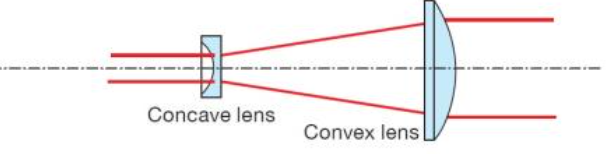
\includegraphics[scale=0.5]{5.png}
			\caption{伽利略型扩束镜}
		\end{figure}
		\item [4.]请调研文献给出一个光信息处理技术的应用例子。
		\item [ ]答:根据空间生命科学与生物技术领域的研究现状及发展情况,
		生命科学实验平台以分子、细胞、组织、个体及群体等不同层次的生物样品
		为研究对象,研究生物样品的生命活动在空间特殊环境下所发生的变化,而生
		物的光信息与生物的生命活动密切相关,因此对这些生物的光信息进行准确、
		高效、针对性强地处理,对生命科学研究起着非常重要的作用\cite{赵青青2017生物光信息处理技术研究}。
	\end{itemize}

	\nocite{*}

	\subsection*{总结与展望}
	本次实验让我更好的了解到了透镜的阿贝成像原理,对其成像过程有了更深刻的认识。刚
	开始做实验时由于理解不够,成像放大倍数不够,导致未能做出有效的结果,在仔细思考后才成功完成实验。
	
	虽然实验总体比较成功,但也留下的一些疑问,对思考题(1)的理解仍然不够,查找文献未能
	找到精确的分析尤其是关于$d = 2a$的分界情况,希望以后能够解决。


	\bibliographystyle{plain}
	\bibliography{Fourier}
	
	
	\label{unknown}
\end{document}